\documentclass{article}
\newsavebox{\oldepsilon}
\savebox{\oldepsilon}{\ensuremath{\epsilon}}
\usepackage[minionint,mathlf,textlf]{MinionPro} % To gussy up a bit
\renewcommand*{\epsilon}{\usebox{\oldepsilon}}
\usepackage[margin=1in]{geometry}
\usepackage{graphicx} % For .eps inclusion
%\usepackage{indentfirst} % Controls indentation
\usepackage[compact]{titlesec} % For regulating spacing before section titles
\usepackage{adjustbox} % For vertically-aligned side-by-side minipages
\usepackage{array, amsmath,  mhchem}
\usepackage[hidelinks]{hyperref}
\usepackage{courier, subcaption}
\usepackage{multirow, enumerate}
\usepackage[autolinebreaks,framed,numbered]{mcode}
\usepackage{float}
\restylefloat{table}

\pagenumbering{gobble} 
\setlength\parindent{0 cm}
\renewcommand{\arraystretch}{1.2}
\begin{document}
\large

MCB 135 Problem Set 6 \hfill Due Wednesday, March 25, 2015 at 2:30 PM

\section*{Problem 1: Band pass filter (55 points)}

As many jet-setters discover, circadian clocks are not useful unless their phase is set appropriately. Entrainment is the process of setting a biological clock's phase in response to external cues such as sunlight. Unfortunately, entrainment cues themselves may be noisy and require filtering.\\

Consider an entrainment system whose input is the ambient light level $x(t)$, which oscillates with 24-hour period but is subject to many sources of variation. The system's output $y(t)$ would ideally be sinusoidal with period 24 hours and the same phase as the circadian signal.\\

\begin{center}
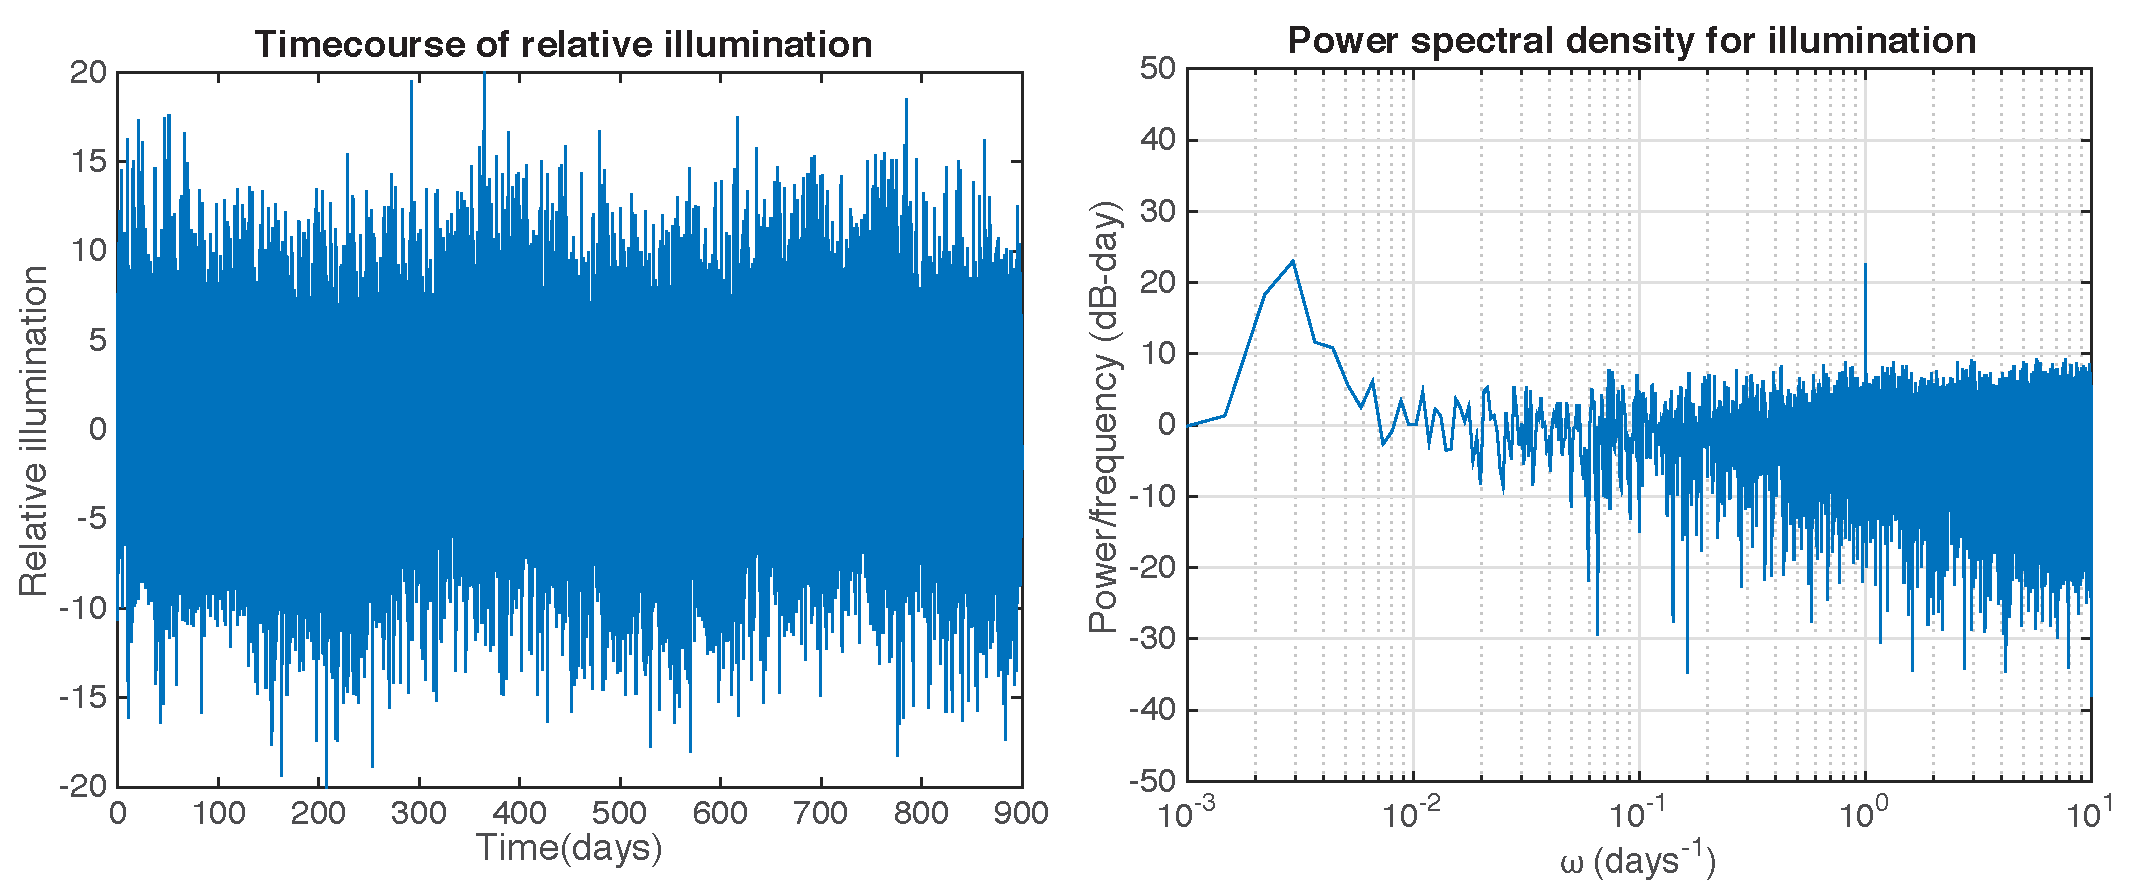
\includegraphics[width=.7\textwidth]{sun.pdf}
\end{center}

The time course at left shows $x(t)$ measurements taken every hour, beginning at noon, for 900 days. $x(t)$ was then decomposed into a combination of sine waves of different frequencies: the \textit{power spectral density }(PSD) plot at right gives the relative power of each wave vs. its frequency, $\omega$. The time course data and code used to generate the PSD are available on the course website.

\begin{enumerate}[a)]
\setlength{\itemsep}{0pt}
\item Which of the two major peaks in the PSD represents the signal we wish to amplify? What is the source of the other peak?
\item Determine the closed loop transfer function for the system depicted below in terms of $K(s)$.

\begin{center}
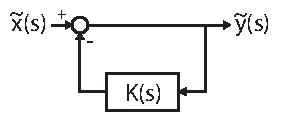
\includegraphics[width=.3\textwidth]{feedback.pdf}
\end{center}


\item What type of controller can be used to preferentially amplify high frequencies? Low frequencies?
\item Combine your answers in part (c) to choose a  form for $K(s)$ so that the closed loop system filters out both high and low frequency noise. Include appropriate units on any constants\footnote{Hint: What is one period in radians? As you complete the remaining questions, it should become clear whether your units were selected properly.}.
\item Construct a Bode plot for your closed loop system. Will the phase of the output be accurate for oscillations with a 24-hour period? \pagebreak
\item Use MATLAB's \mcode{lsim()} function with the time course data and your closed loop transfer function to simulate the output of your system, $y(t)$. Include plots of $y(t)$ with appropriate windows to:
\begin{itemize}
\item Confirm that your system's output is dominated by oscillations with a 24-hour period.
\item Show the range of variation in amplitude over 900 days.
\item Indicate the ``burn-in" time, i.e., time elapsed before the system's output has reasonably steady phase and amplitude.
\end{itemize} 
\item Are there trade-offs between shorter burn-in time and variation in amplitude for the system you've designed? Demonstrate your conclusion by showing a plot with a different choice of parameters.
\item Simulate a ``free run" by setting $x(t)$ to zero at some time after the burn-in. How long does your system continue to oscillate appreciably?
\end{enumerate}

\section*{Problem 2: Resonator (25 points)}

An alternative approach to amplify oscillations at a frequency of interest uses resonant systems. Consider the following system of two transcription factors, $A$ and $B$: expression of $A$ is driven by an input signal $x(t)$ but is repressed by $B$. $A$ activates expression of $B$. Both transcription factors are subject to dilution/degradation.

\begin{eqnarray*}
\frac{da}{dt} & = & x(t) - k b - \gamma a\\
\frac{db}{dt} & = & ka - \gamma b
\end{eqnarray*}

The output of this system is regarded to be the concentration $a(t)$.

\begin{enumerate}[a)]
\setlength{\itemsep}{0pt}
\item Apply a Laplace transformation to the system and rearrange to find the system's closed loop transfer function, $\frac{\tilde{a}(s)}{\tilde{x}(s)}$.
\item Prepare a Bode plot of this system with $\gamma=0.002 \pi $, $k=2\pi$.
\item Repeat problem 1f using the resonator transfer function. Compare the result to your band pass filter's output.
\end{enumerate}

\section*{Problem 3: Alternative coherent feedforward loop (adapted from Alon 4.5, 20 points)}

\begin{minipage}[b]{0.1\linewidth}
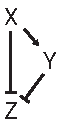
\includegraphics[width=\textwidth]{c3ffl.pdf}
\end{minipage}
\hspace{0.5cm}
\begin{minipage}[b]{0.85\linewidth}
Solve the dynamics of the type-3 coherent FFL (shown at left), assuming AND logic at the $Z$ promoter, in response to (i) a step increase and (ii) a step decrease in the concentration of $X$. Here, AND logic means that $Z$ is produced only if both $X$ and $Y$ are below their threshold concentrations for promoter binding. Are there delays? What logic gate does this circuit embody at steady-state? Compare your answers to the type-1 coherent FFL described in class.\\

\end{minipage}



\end{document}